\documentclass[14pt]{extreport}
\usepackage{gost}
\usepackage{hyperref}
\usepackage{makecell}
\usepackage{ragged2e}
\usepackage{graphicx}%Вставка картинок правильная
\usepackage{float}%"Плавающие" картинки
\usepackage{wrapfig}%Обтекание фигур (таблиц, картинок и прочего)
\justifying
\makeatletter
\@addtoreset{figure}{part}% Reset figure numbering at every part
\makeatother
\renewcommand{\thefigure}{\arabic{figure}}% Figure number is part.figure
\renewcommand{\thetable}{\arabic{table}}
\setcounter{secnumdepth}{3}


%Тут можно вставить дополнительные пакеты

\begin{document}
\pagestyle{empty} %  выключаем нумерацию
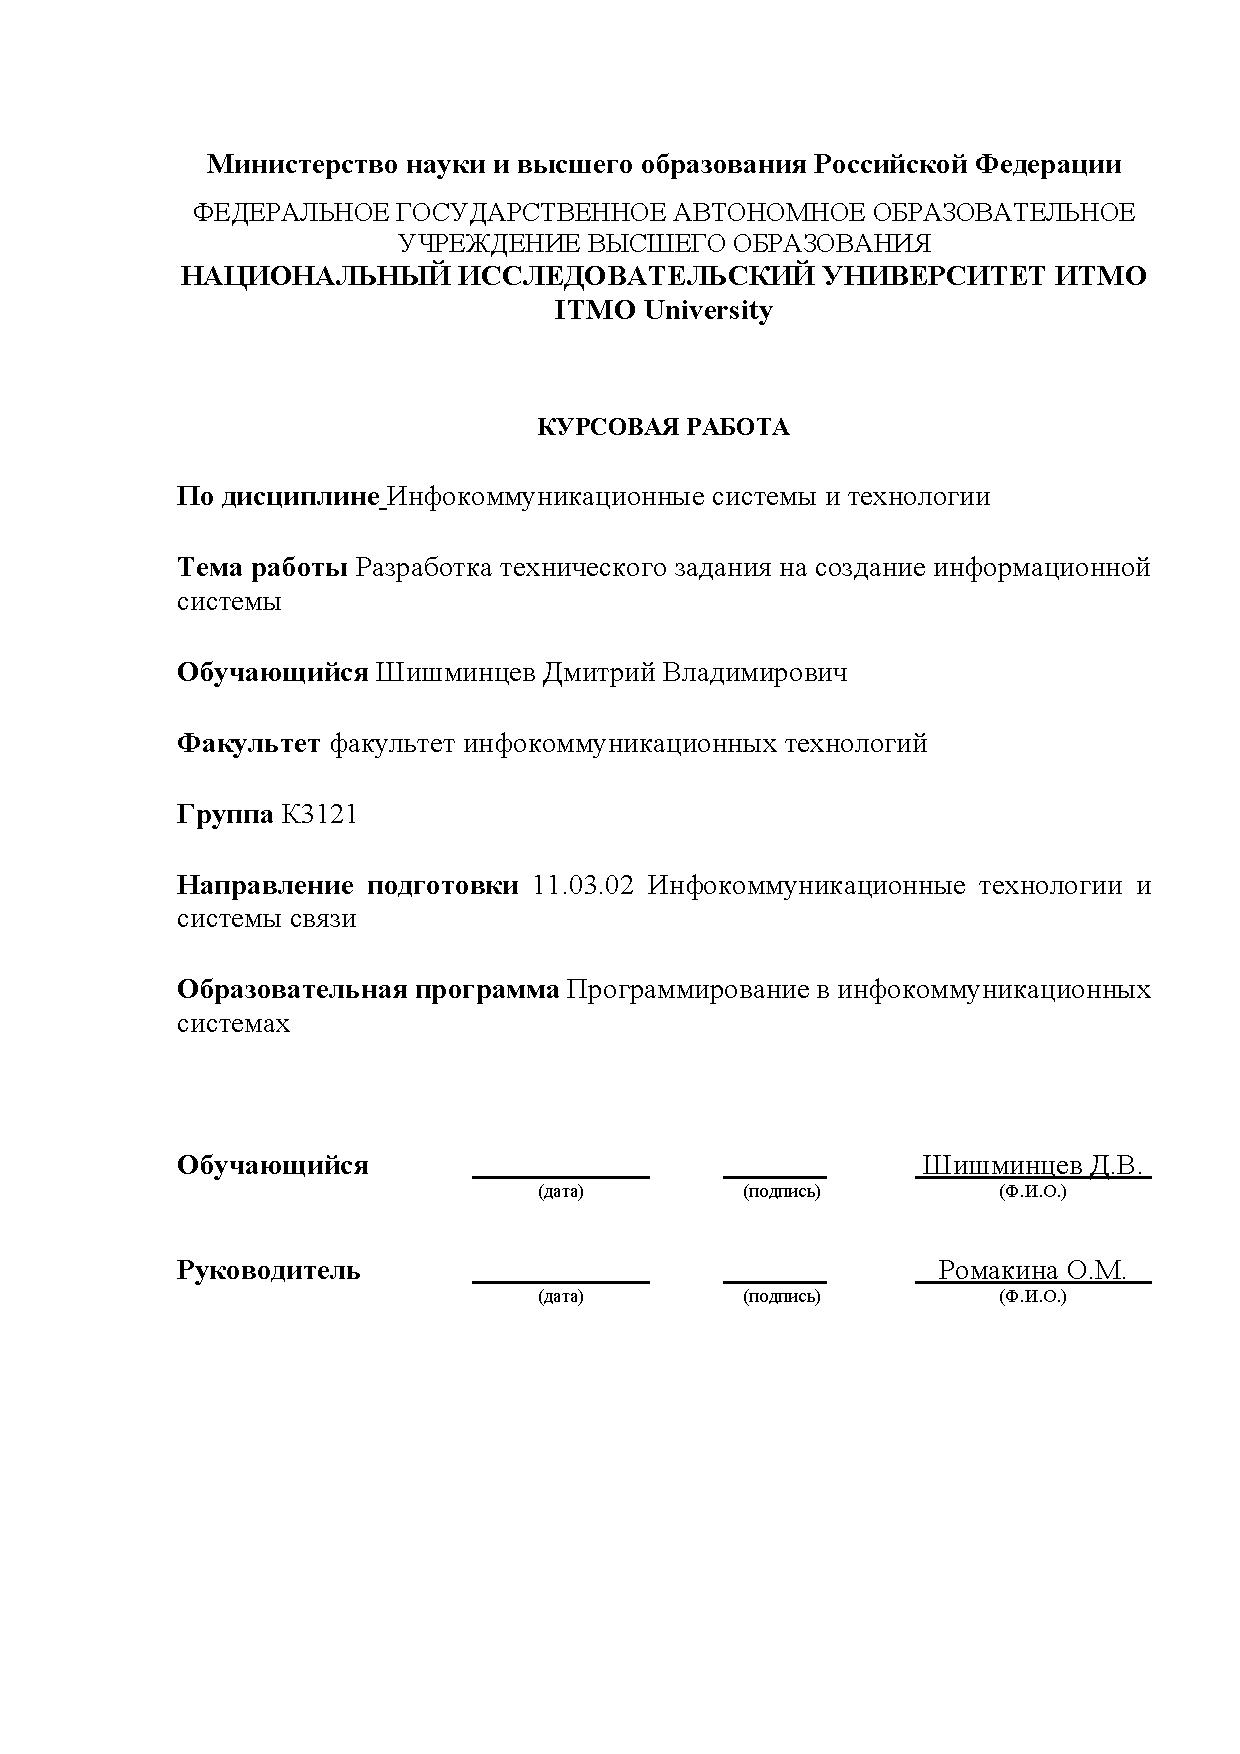
\includepdf[pages=-,pagecommand={}]{title_page.pdf}

\pagestyle{plain} % включаем нумерацию
\newpage
\begin{center}
\begin{normalsize}
\textbf{АННОТАЦИЯ}
\end{normalsize}
\end{center}

Тема курсового проекта: Разработка технического задания на создание мобильного приложения.

Выполнил - Шишминцев Д. В.

Руководитель - Ромакина О. М. 

Работа состоит из двух глав, заключения и списка используемых источников. (7 наименований)

В введении поставлена цель и задачи курсовой работы, обоснована актуальность работы. 

В первой главе описана предметная область, необходимые функции системы, анализ рынка, разработаны UML, DFD, IDEF0, IDEF3, BPMN диаграммы для будующей системы. 

Во второй главе представлено техническое задание на разработку инфокоммуникационной системы. 

В заключении представлены выводы, полученные в результате написания курсовой работы. 

Ключевые слова: анализ рынка, проектирование, функциональные модели, диаграммы, техническое задание

Работа состоит из 41 страницы, содержит 18 рисунков. 
\newpage

\tableofcontents
\intro\label{intro} 

Актуальность выбранной темы инфокоммуникационной системы обусловлена тем, что в настоящее время людей окружает куда больше информации, чем в прошлом веке. У людей больше различных дел, и договориться о встрече с другими людьми крайне сложно, особенно сложно держать всю эту информацию в голове. Из за этого появляется спрос на системы планирования времени. 

В настоящее время на рынке представлены системы планирования личного времени, но в этих системах не учитывается расписание пользователей с которыми человек контактирует.

Решением этой проблемы может стать разработка веб-приложения MEET ME. Приложение позволяет пользователям смотреть пересечения расписаний с их друзьями и коллегами и позволяет упростить планирование встреч. Следовательно, тема действительно актуальна и дальнейшая разработка имеет смысл.

Целью данной работы является разработка технического задания веб-приложения MEET ME. 

Исходя из цели работы, были поставлены следующие задачи:
\begin{itemize}
    \item описать идею системы;
    \item провести анализ рынка;
    \item разработать диаграммы согласно стандартам UML, IDEF0, IDEF3, DFD, BPMN для описания принципов функционирования системы;
    \item создать техническое задание на разработку инфокоммуникационной системы;
\end{itemize}





% ////////////////////////////////////////////////////////
%                     ЛАБА 3
% ////////////////////////////////////////////////////////



\chapter{Анализ предметной области}


    \section{Описание идеи инфокоммуникационной системы \label{chapter1}}

        \subsection{Основной функционал }

        Информационная система MEET ME представляет из себя веб-приложение для планирования встреч с друзьями и родственниками в виде календаря. 
        Приложение показывает пересечение свободного времени пользователя с одним или несколькими его друзьями.
        C помощью данного приложения пользователь может эффективно планировать встречи со своими друзьями, родственниками или знакомыми не тратя огромное количество времени на согласования времени. 

        После создания аккаунта, пользователю будет предложено настроить свое расписание. Пользователь выбирает дни и время, когда он имеет возможность для встречи. Планируется реализация возможности определения свободных промежутков с помощью импорта данных с Google Calendar и аналогов, а так же .cal файлов.
        Пользователь может настроить свое расписание как на неделю, так и на месяц вперед. Настроив свое расписание, пользователь должен добавить своих друзей.  Добавление друзей идет посредством отправки запроса другу на его электронную почту указаную при регистрации аккаунта. Добавив своих друзей, пользователь может создать группу из друзей, если они планируют встречаться вместе.

        Настроив свое расписание и добавив друзей, пользователю начинают отображаться пересечения в расписании с его друзьями в виде календаря. Пользователю не показывается полностью расписание встреч его друзей ради сохранения приватности. Пользователь может отправить приглашение на встречу своему другу если их свободное время пересекается в приложении. Приглашение отобразится у его друга и он сможет принять или отклонить его. Приняв приглашение у обоих пользователей отобразится встреча в их календаре. Так же пользователь может создать группу из друзей. Создав группу, она будет отображаться в пересечениях вместе с друзьями. Рядом с названием группы будет отображаться количество друзей из группы, для которых это врем свободно. Участники группы могут утвердить время встречи методом голосования и тогда встреча будет отображаться в расписании остальных участников группы, они смогут присоединиться к мероприятию нажав на соответствующую кнопку.

        Подводя итоги, приложение будет иметь следующий функционал 
        \begin{itemize}
            \item Регистрация аккаунта;
            \item Настройка свободного времени вручную;
            \item Настройка свободного времени основываясь на рекомендациях данных системой благодаря импорту расписания из Google Calendar / .cal файлов;
            \item Редактирование свободного времени;
            \item Отправка и принятие заявок в друзья;
            \item Создание группы из существующих друзей;
            \item Отправка приглашений на встречу;
            \item Принятие/Отклонение встречи;
            \item Утверждение групповой встречи методом голосования.
        \end{itemize}
        \subsection{Основные пользователи  }

        Информационная система будет иметь только прямых конечных пользователей. Система не требует модераторов, менеджеров и прочих пользователей.
        Целевая аудитория данной информационной системы достаточно широка. Основными пользователями будут молодые, общительные люди, которые стараются грамотно распределять свое время (ученики старших классов, студенты, работающая молодежь).

        \newpage
        \subsection{Прототип интерфейса}
        В данном разделе демонстрируется прототип веб-приложения для компьютеров (Рисунок \ref{fig:prototype}). Интерфейс состоит из боковой панели, календаря и элементов управления. На боковой панели присутствует название приложения, кнопка <<изменить>>, которая позволяет изменять собственное расписание, список друзей, кнопка позваляющая добавить нового друга. Ниже располагается список компаний, а так же кнопка позоляющая создать новую. При наличии активных приглашений, они будут отображаться снизу. Их можно будет принять или отклонить нажав на соответствующую кнопку.
        Сверху находятся элементы управления. Пользователь может выбрать отображение календаря на неделю, месяц или 3 дня. Используя соответствующие кнопки пользователь может перемещаться на выбранный период. Так же сверху находятся настройки аккаунта, в которые пользователь может попасть кликнув на свое имя.
        \begin{figure}[h]   
            \centering
            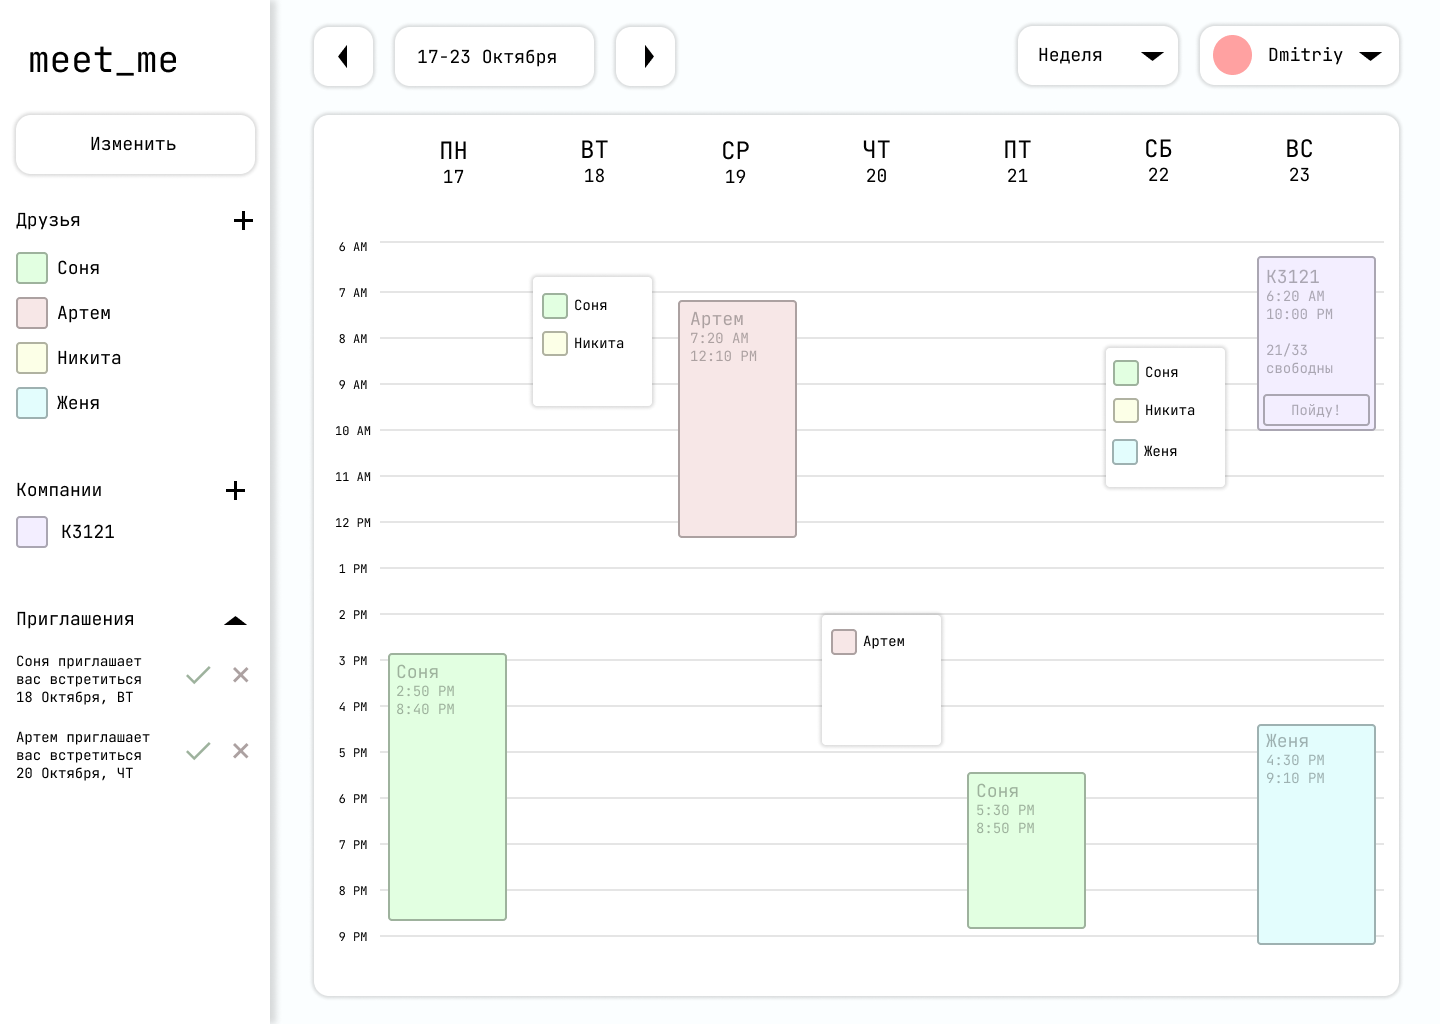
\includegraphics[width=0.9\linewidth]{./img/prototype.png}
            \caption{ Прототип интерфейса}
            \label{fig:prototype}
        \end{figure}

        Основная часть интерфейса выполнена в виде календаря. Календарь размечен по дням и времени.
        На календаре, тем же цветом, что и в боковой панели, отображаются уже согласованные встречи с друзьями. Белым же цветом отображаются пересечения свободного времени с друзьями. В блоке пересечений отображаются друзья, с которыми свободное время пересекается.
        Нажав на имя друга, пользователю будет предложено отправить приглашение другу на это свободное время.

    \section{Анализ рынка \label{chapter2}}
        \subsection{Обзор аналогов, представленных на рынке}
        Проведя анализ российского и зарубежного рынка, аналогов обнаружено не было. Существует несколько систем имеющих частично похожий функционал. 
        В отличии от представленных ниже систем, система представленная в данном отчете ориентируется на использование людьми для ведения их личной жизни, а не для рабочих нужд. Так же система не завязана на одном пользователе создавшем опрос и может равноправно использоваться всеми участниками.
        \subsubsection{NeedToMeet}
        Сервис NeetToMeet \eqref{a:NeetToMeet} предоставляет возможность пользователям создавать опросы, благодаря которым можно выбрать время и место для встречи. Сервис предоставляет ограниченное количество возможностей в бесплатной версии, полная версия стоит 20\$/год. Сервис в основном ориентируется на корпоративный сегмент. 
        \subsubsection{Rally}
        Сервис Rally \eqref{b:Rally} имеет схожих функционал с сервисом NeedToMeet, но в отличии от него бесплатен, имеет открытый исходный код, а так же для его использования не нужно регистрировать аккаунт. Пользователь так же создает опрос, а другие пользователи выбирают удобное время для встречи. 
        \subsubsection{WhenAvalible}
        Используя сервис WhenAvalible \eqref{c:WhenAvalible} пользователь создает опрос, а другие пользователи подтверждают свою возможность встретиться в тот или иной день. Сервис предоставляет ограниченный функционал в бесплатной версии, платная версия стоит 38\$/год.

        \subsection{Обоснование необходимости разработки информационной системы }
        Проведя анализ рынка, можно сделать вывод, что идея уникальна. Аналогов на рынке не найдено, а те сервисы, что имеют частично схожий функционал - завязаны вокруг одного пользователя, который создает опрос. 

        

% ////////////////////////////////////////////////////////
%                     ЛАБА 5
% ////////////////////////////////////////////////////////


\newpage

    \section{Разработка диаграмм прецедентов и диаграмм активности }

        \subsection{Диаграмма прецедентов}
        В данном разделе демонстрируется диаграмма прецедентов [\ref{fig:uml1}]  для будующей информационной системы. Диаграмма описывает систему на концептуальном уровне и позволяет понять ее возможности и отношение с актерами.
        \begin{figure}[h]   
            \centering
            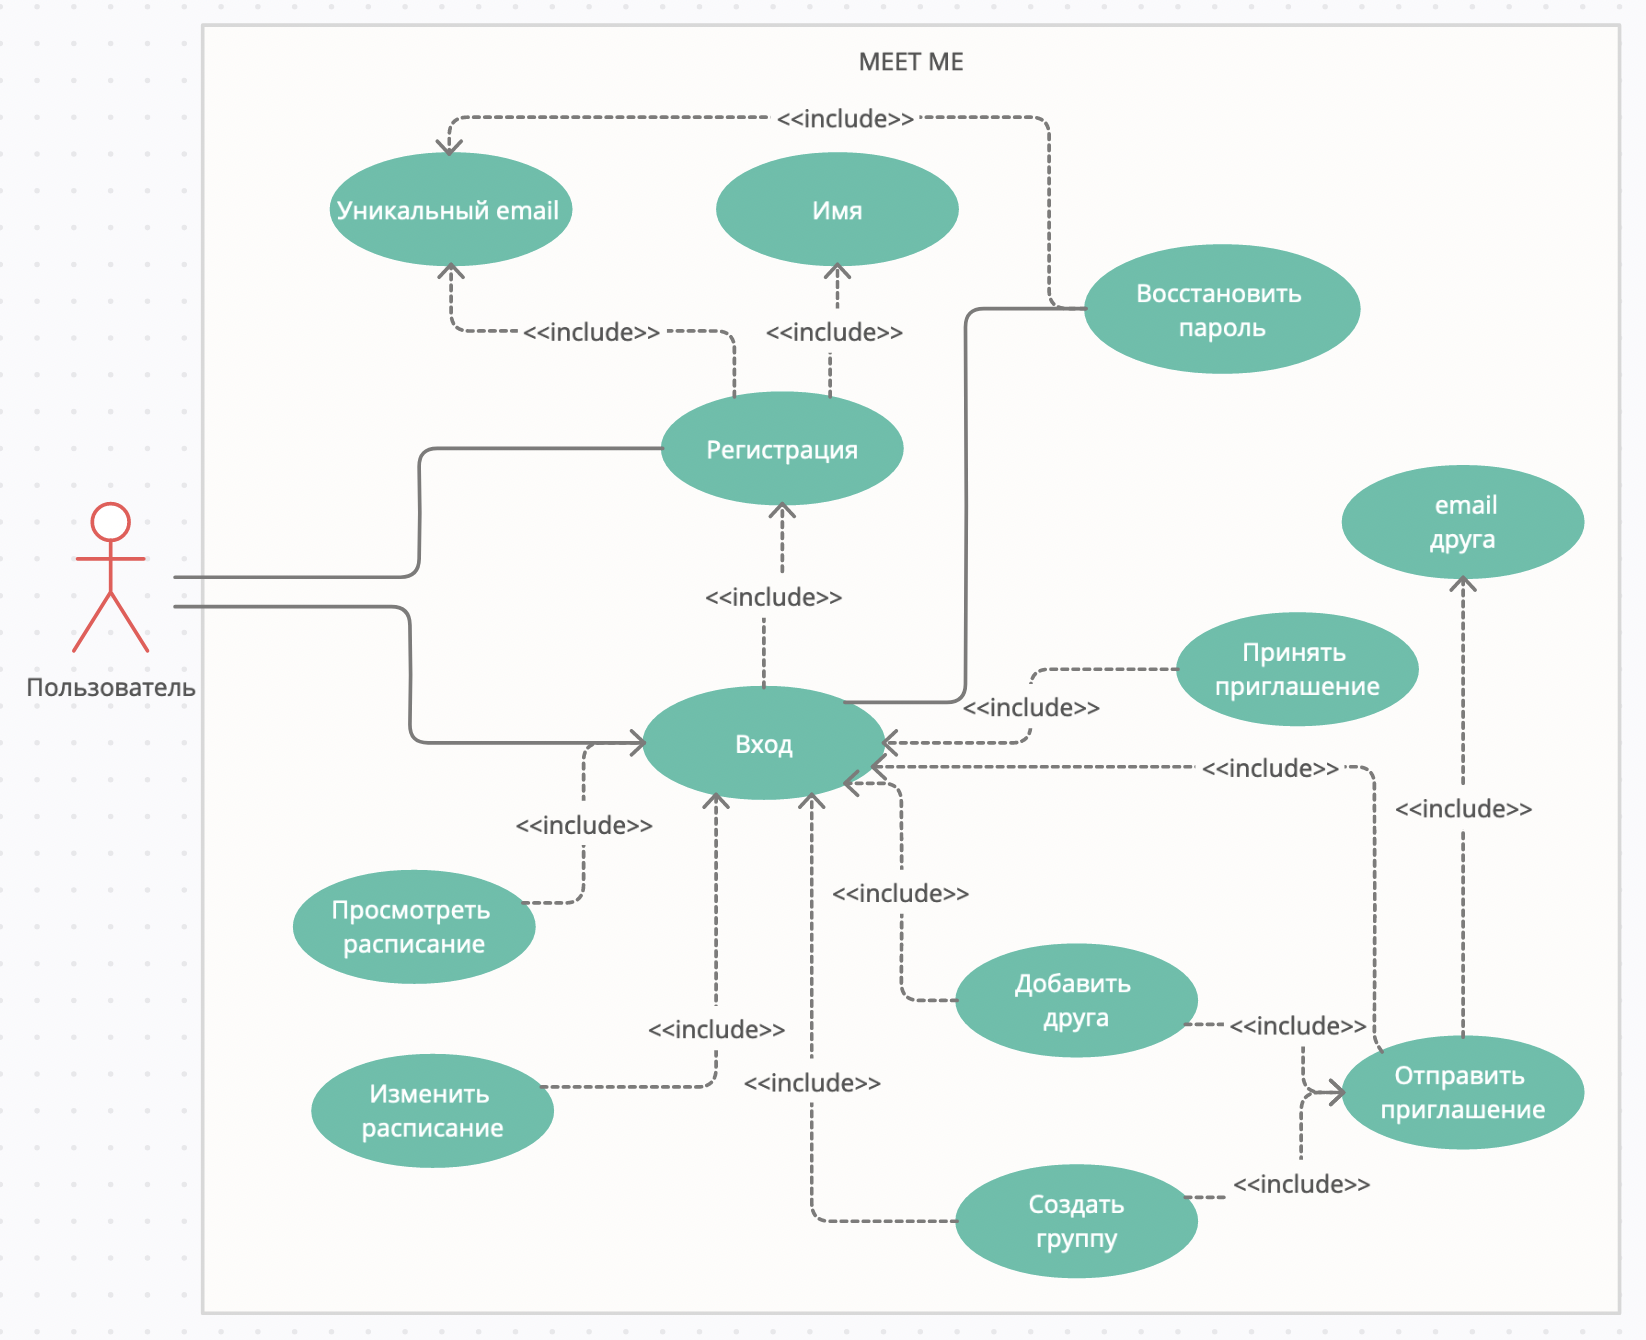
\includegraphics[width=0.8\linewidth]{img/d1.png}
            \caption{ Диаграмма прецедентов}
            \label{fig:uml1}
        \end{figure}
        
        \subsection{Диаграммы активности для ключевых прецедентов}
        Для ключевых прецедентов были составлены диаграммы активности. Представленные диаграммы отражают динамические аспекты поведения системы.
        
        Диаграмма прецедента <<Вход>> [\ref{fig:uml2}] показывает поведение системы при входе пользователя в систему. Если пользователь не зарегистрирован, то система предложит ему создать аккаунт. Если пользователь не может войти в систему, то система предложит ему восстановить пароль.
        \begin{figure}[h]   
            \centering
            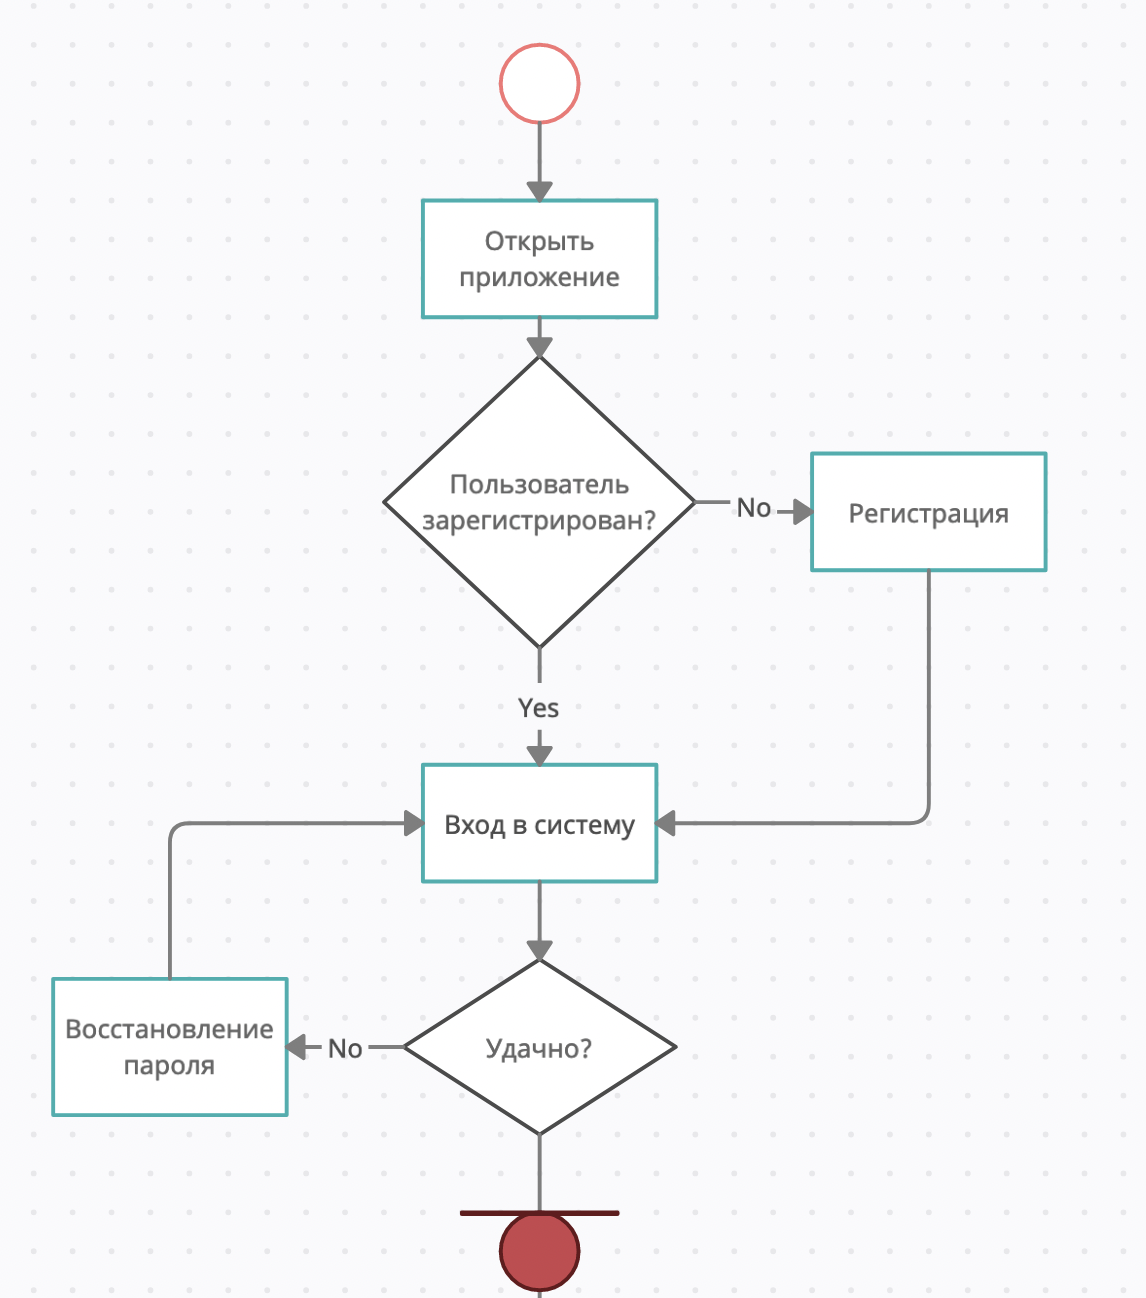
\includegraphics[width=0.94\linewidth]{img/d2.png}
            \caption{ Диаграмма прецедента <<Вход>>}
            \label{fig:uml2}
        \end{figure}
        \newpage 
        Диаграмма прецедента <<Просмотреть расписание>> [\ref{fig:uml3}] показывает поведение системы при отображении расписания. Если расписание не настроено, то пользователю предложат его настроить. Система отображает запланированные встречи, если они есть, далее если есть пересечения свободного времени с друзьями, то показывает блоки пересечения. 
        \begin{figure}[h]   
            \centering
            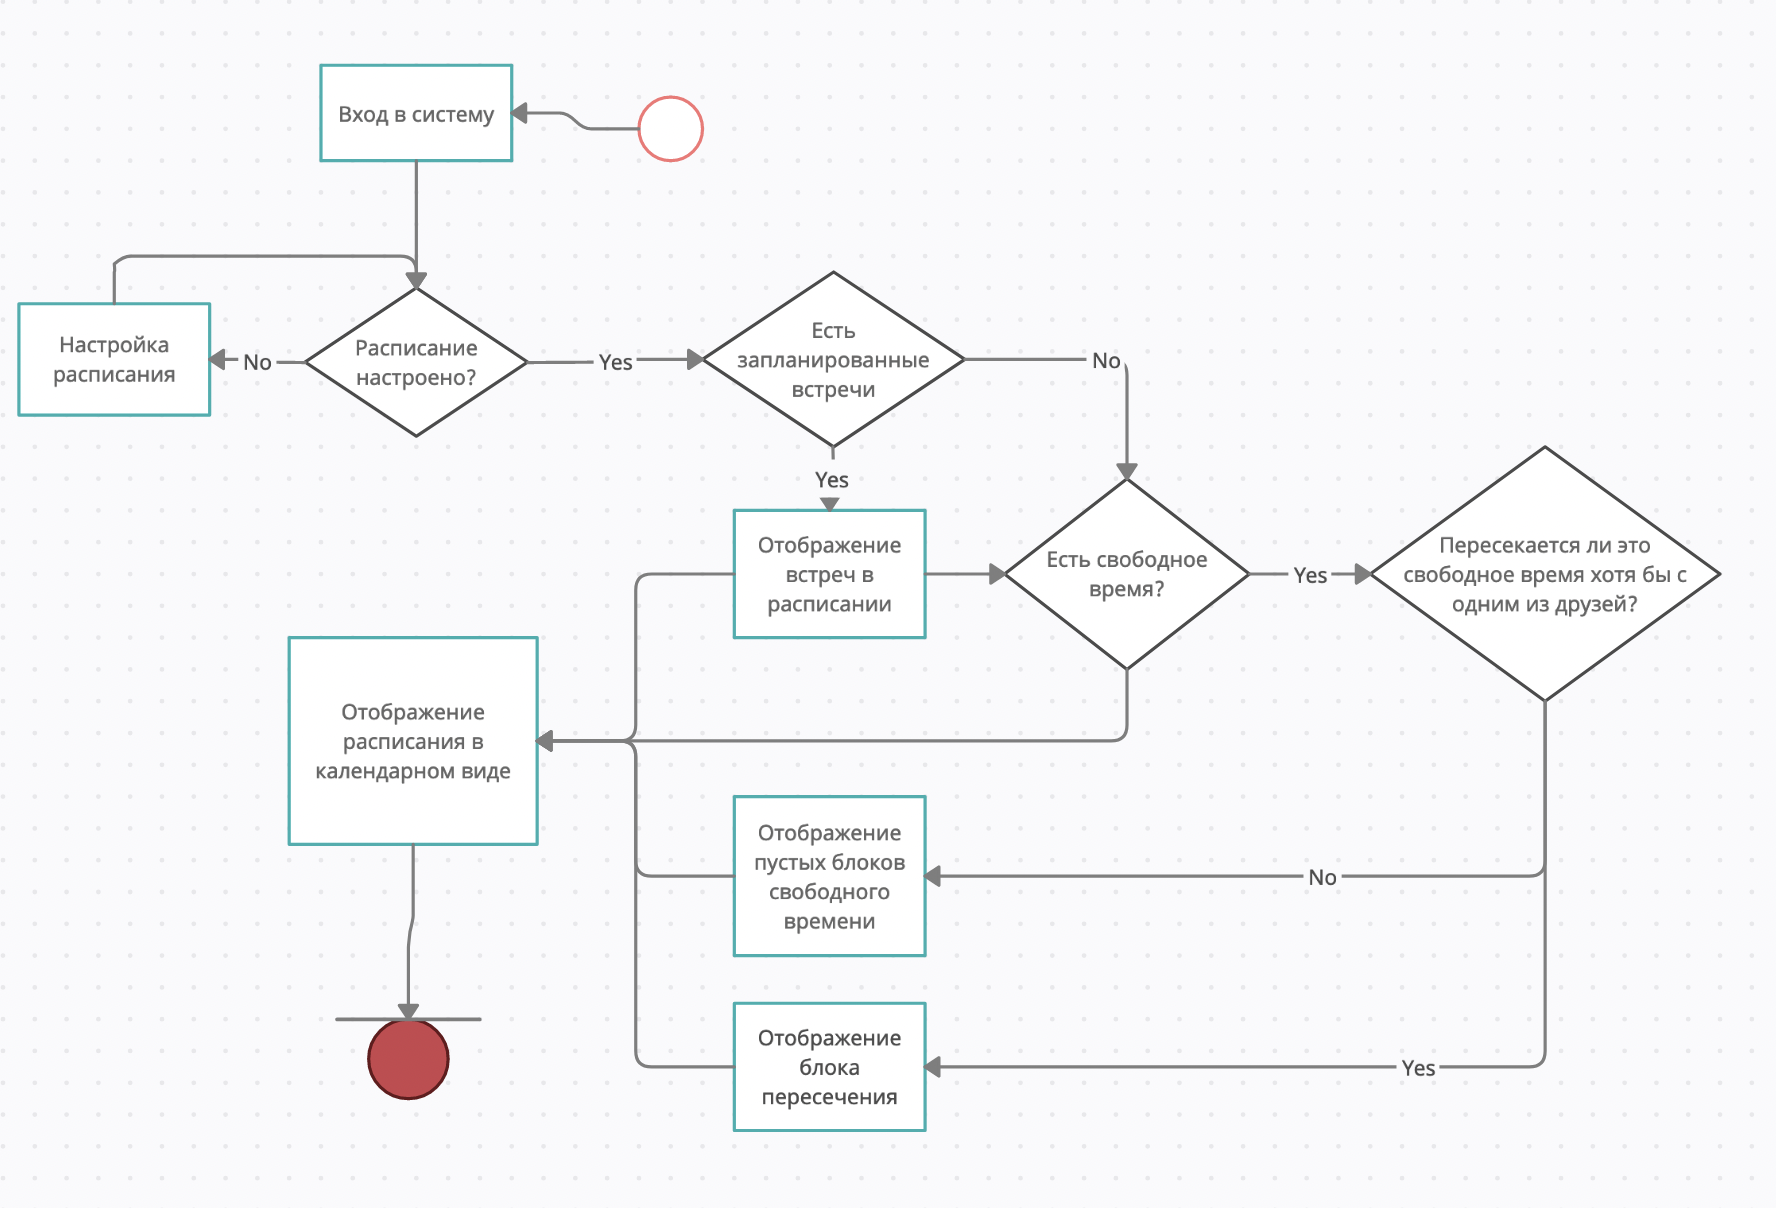
\includegraphics[width=0.94\linewidth]{img/d3.png}
            \caption{ Диаграмма прецедента <<Просмотреть расписание>>}
            \label{fig:uml3}
        \end{figure}
        
        
        \subsection{Альтернативные потоки и исключения}
        Для представленных диаграмм рассмотрены альтернативные потоки и исключения в виде таблиц. Таблица \ref{table1} для диаграммы прецедента <<Вход>>, а так же таблица \ref{table2} для диаграммы <<Просмотр расписания>>
        
        \begin{table}[H]
        
            \begin{center}
            \caption{Вход \label{table1}}
            \begin{tabular}{|p{5.5cm}|p{10.7cm}|}
            \hline
            Вариант использования & Вход \\
            \hline
            Актеры
             & Пользователь
             \\
            \hline
            Цель
             & Вход в систему для получения доступа к расписанию 
             \\
            \hline
            Краткое описание
             & Система требует пользователя войти в существующий аккаунт или создать новый 
             \\
            \hline
            Исключения
             & 
            $\cdot$ Аккаунт с введенным адресом электронной почты уже существует 
            
            $\cdot$ Пользователь не прошел проверку на робота 
             \\
            \hline
            Альтернативный ход 
            
            событий
            & Пользователь может закончить использование системы \\
            
            \hline
            \end{tabular}
            \end{center}
            \end{table}
        
        
            \begin{table}[H]
        
                \begin{center}
                \caption{Просмотр расписания \label{table2}}
                \begin{tabular}{|p{5.5cm}|p{10.7cm}|}
                \hline
                Вариант использования & Просмотр расписания \\
                \hline
                Актеры
                 & Пользователь
                 \\
                \hline
                Цель
                 & Просмотр расписания с целью создания встречи 
                 \\
                \hline
                Краткое описание
                 & Система отображает пользователю пересечение его расписания с его друзьями 
                 \\
                \hline
                Исключения
                 & 
                $\cdot$ У пользователя может быть пустой список друзей 
                
                $\cdot$ У друзей пользователя может быть не настроено расписание 
                 \\
                \hline
                Альтернативный ход 
                
                событий
                & Пользователь может добавить себе других друзей \\
                
                \hline
                \end{tabular}
                \end{center}
                \end{table}
            


% ////////////////////////////////////////////////////////
%                     ЛАБА 6
% ////////////////////////////////////////////////////////
\newpage 


\section{Разработка диаграмм IDEF0, DFD, IDEF3, BPMN для будующей инфокоммуникационной системы}

\subsection{Функциональные модели по стандарту IDEF0}
В данном разделе представлены функциональные модели по стандарту IDEF0. Изучив стандарт IDEF0 (учебное пособие \ref{bib:bib1}), была разработана контекстная диаграмма (рисунок \ref{fig:idef01}), декомпозиция контекстной диаграммы (рисунок \ref{fig:idef02}),  декомпозиция блока <<Авторизация>> (рисунок \ref{fig:idef03}), декомпозиция блока <<Определение общего свободного времени>> (рисунок \ref{fig:idef04}), декомпозиция блока <<Определение расписания пользователя>> (рисунок \ref{fig:idef05}).
\begin{landscape}
    \begin{figure}[h]   
        \centering
        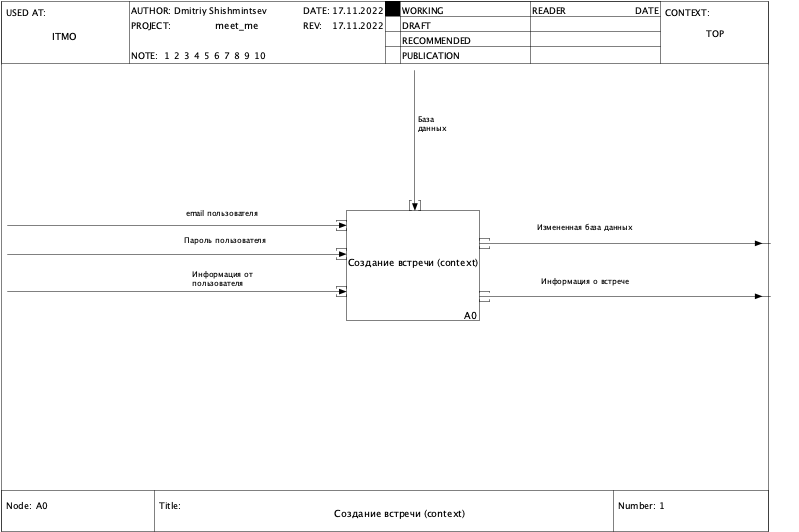
\includegraphics[width=1\linewidth]{img/01_A0.png}
        \caption{ Контекстная диаграмма}
        \label{fig:idef01}
    \end{figure}
    \begin{figure}[h]   
        \centering
        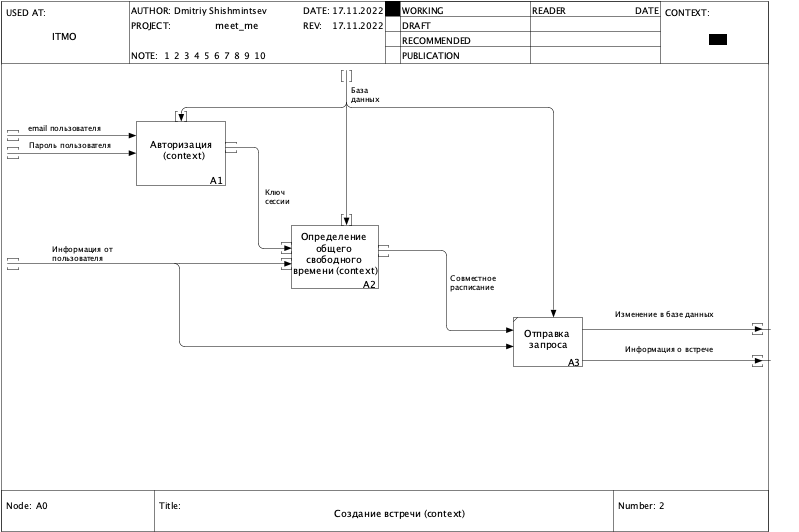
\includegraphics[width=1\linewidth]{img/02_A0.png}
        \caption{ Декомпозиция контекстной диаграммы}
        \label{fig:idef02}
    \end{figure}
    \begin{figure}[h]   
        \centering
        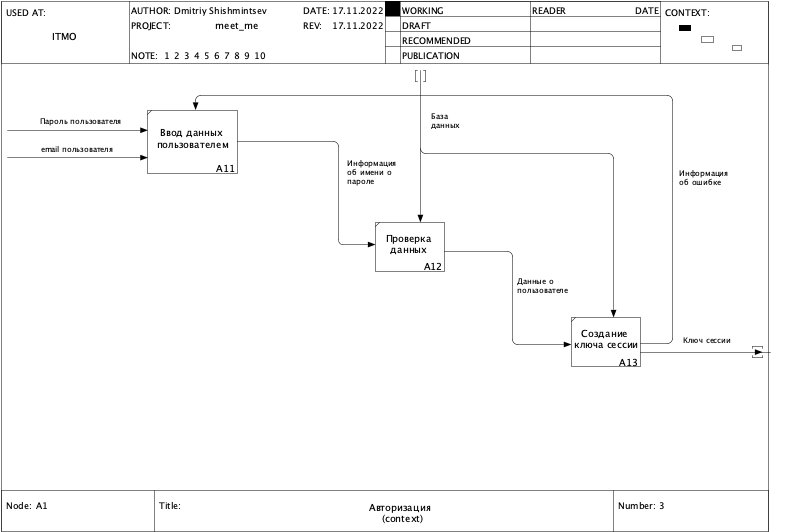
\includegraphics[width=1\linewidth]{img/03_A1.png}
        \caption{ Декомпозиция блока <<Авторизация>>}
        \label{fig:idef03}
    \end{figure}
    \begin{figure}[h]   
        \centering
        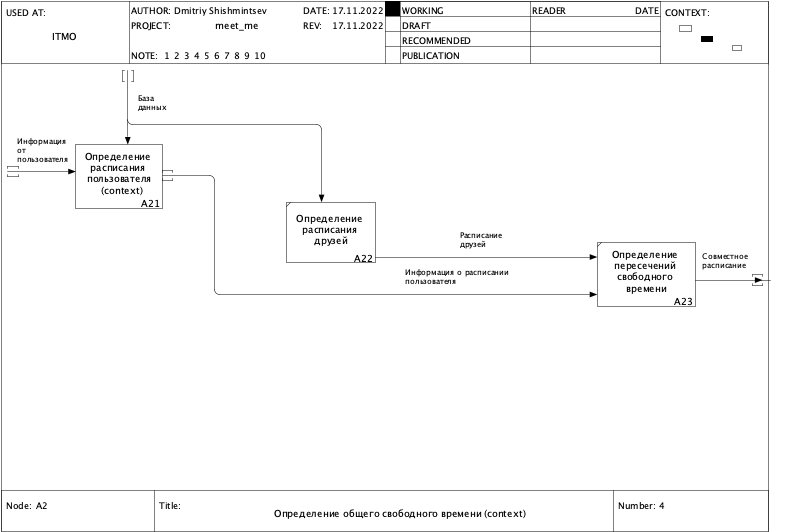
\includegraphics[width=1\linewidth]{img/04_A2.png}
        \caption{ Декомпозиция блока <<Определение общего свободного времени>>}
        \label{fig:idef04}
    \end{figure}
    \begin{figure}[h]   
        \centering
        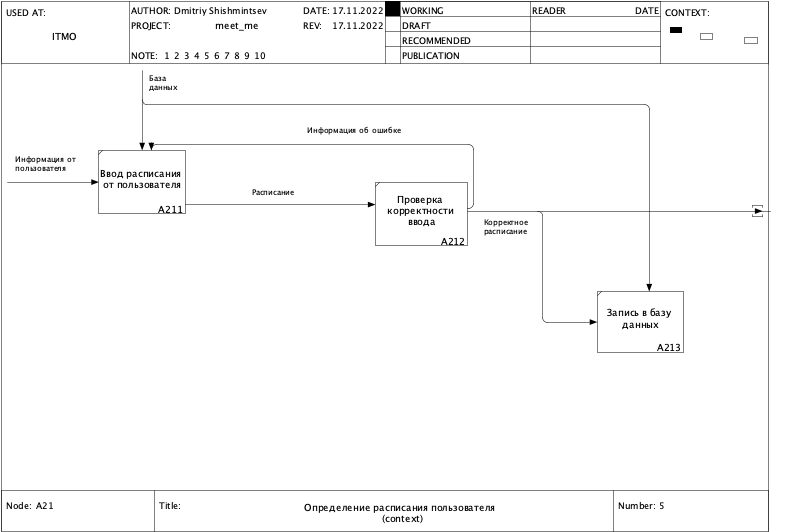
\includegraphics[width=1\linewidth]{img/05_A21.png}
        \caption{ Декомпозиция блока <<Определение расписания пользователя>>}
        \label{fig:idef05}
    \end{figure}
    
\end{landscape}





% ////////////////////////////////////////////////////////
%                     ЛАБА 7
% ////////////////////////////////////////////////////////

\section{Модели по стандарту DFD}
В данном разделе, в качестве дополнения к функциональной модели инфомрационной системы по стандарту IDEF0, представлены диаграммы по стандарту DFD. Для контекстной диаграммы IDEF0 (рисунок \ref{fig:dfd1}) представлена декомпозиция (рисунок \ref{fig:dfd2}). Для блоков <<Авторизация>> и <<Определение общего свободного времени>> представлены диаграммы в стандарте DFD (рисунок \ref{fig:dfd3}, рисунок \ref{fig:dfd4}).

\begin{landscape}
    \begin{figure}[h]   
        \centering
        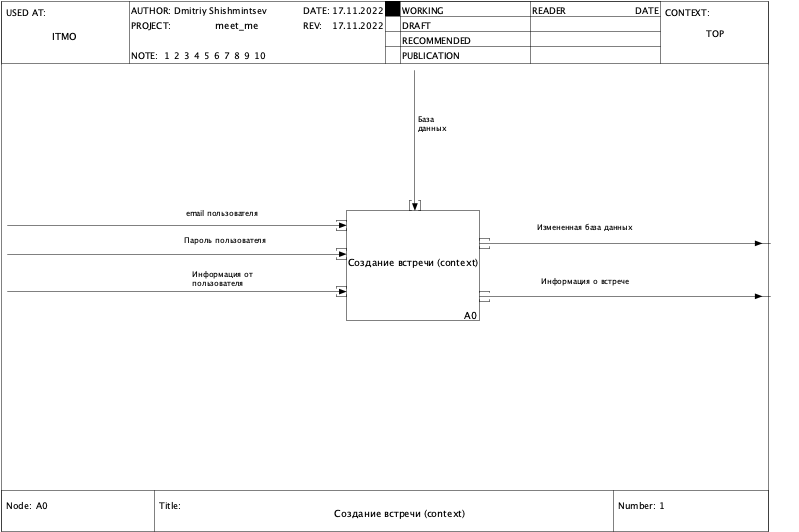
\includegraphics[width=0.9\linewidth]{img/IDEF0-0.png}
        \caption{ Контекстная диаграмма по стандарту IDEF0}
        \label{fig:dfd1}
    \end{figure}

    \begin{figure}[h]   
        \centering
        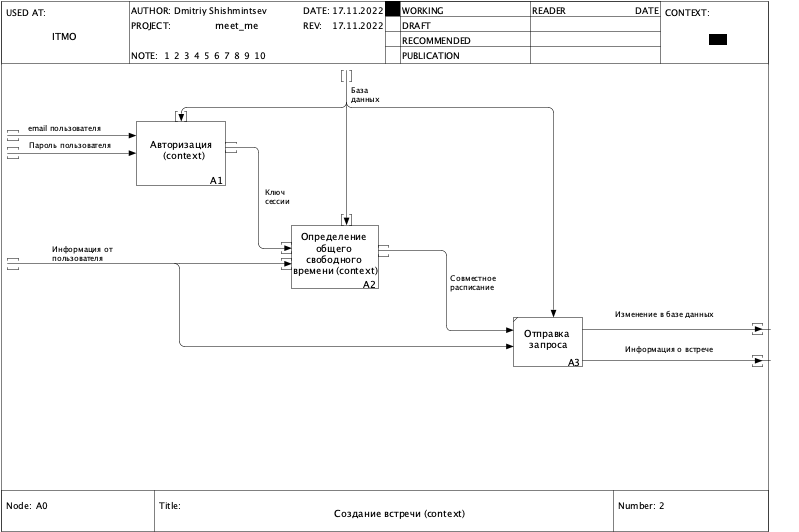
\includegraphics[width=0.9\linewidth]{img/IDEF0-1.png}
        \caption{ Декомпозиция контекстной диаграммы по стандарту IDEF0}
        \label{fig:dfd2}
    \end{figure}

    \begin{figure}[h]   
        \centering
        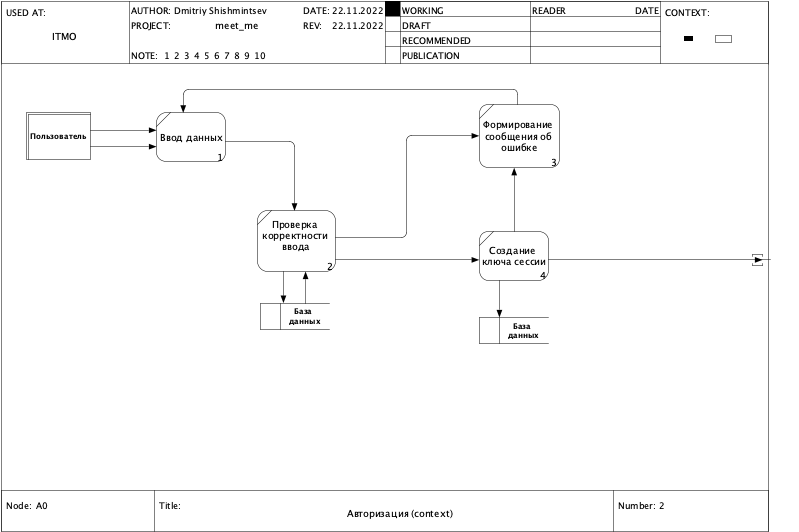
\includegraphics[width=0.9\linewidth]{img/DFD1.png}
        \caption{ Декомпозиция блока <<Авторизация>> по стандарту DFD}
        \label{fig:dfd3}
    \end{figure}

    \begin{figure}[h]   
        \centering
        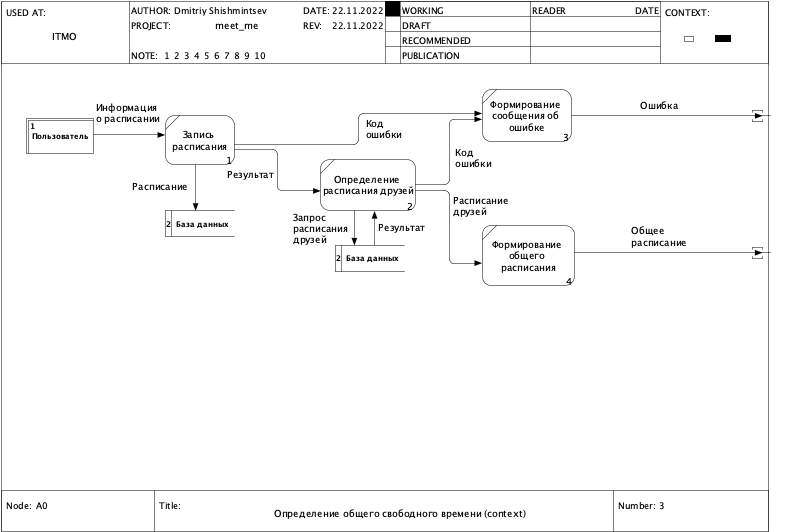
\includegraphics[width=0.9\linewidth]{img/DFD2.png}
        \caption{ Декомпозиция блока <<Определение общего свободного времени>> по стандарту DFD}
        \label{fig:dfd4}
    \end{figure}
\end{landscape}

\section{Модели по стандарту IDEF3}
В данном разделе представлена контекстная диаграмма (рисунок \ref{fig:idef31}), декомпозиция контекстой диаграммы (рисунок \ref{fig:idef32}), декомпозиция блока <<Вход>> (рисунок \ref{fig:idef33}), а так же декомпозиция блока <<Определение общего расписания>> (рисунок \ref{fig:idef34}) согласно стандарту IDEF3. 
\begin{landscape}
    \begin{figure}[h]   
        \centering
        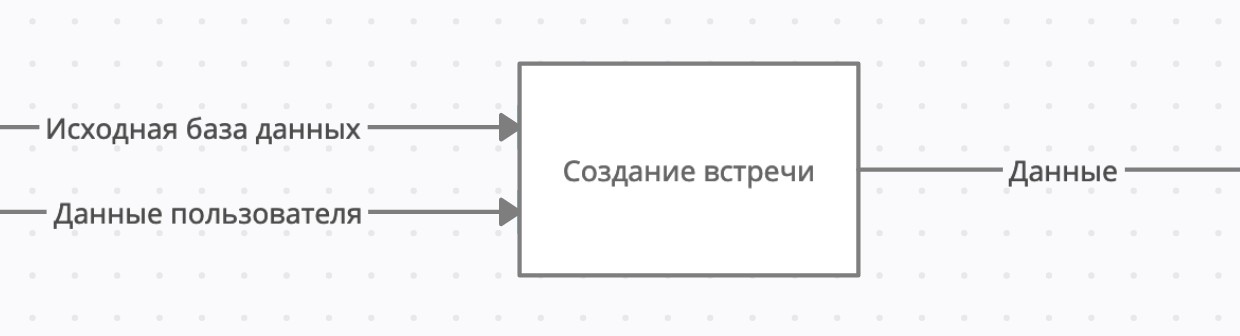
\includegraphics[width=0.7\linewidth]{img/IDEF3-0.png}
        \caption{ Контекстная диаграмма по стандарту IDEF3}
        \label{fig:idef31}
    \end{figure}

    \begin{figure}[h]   
        \centering
        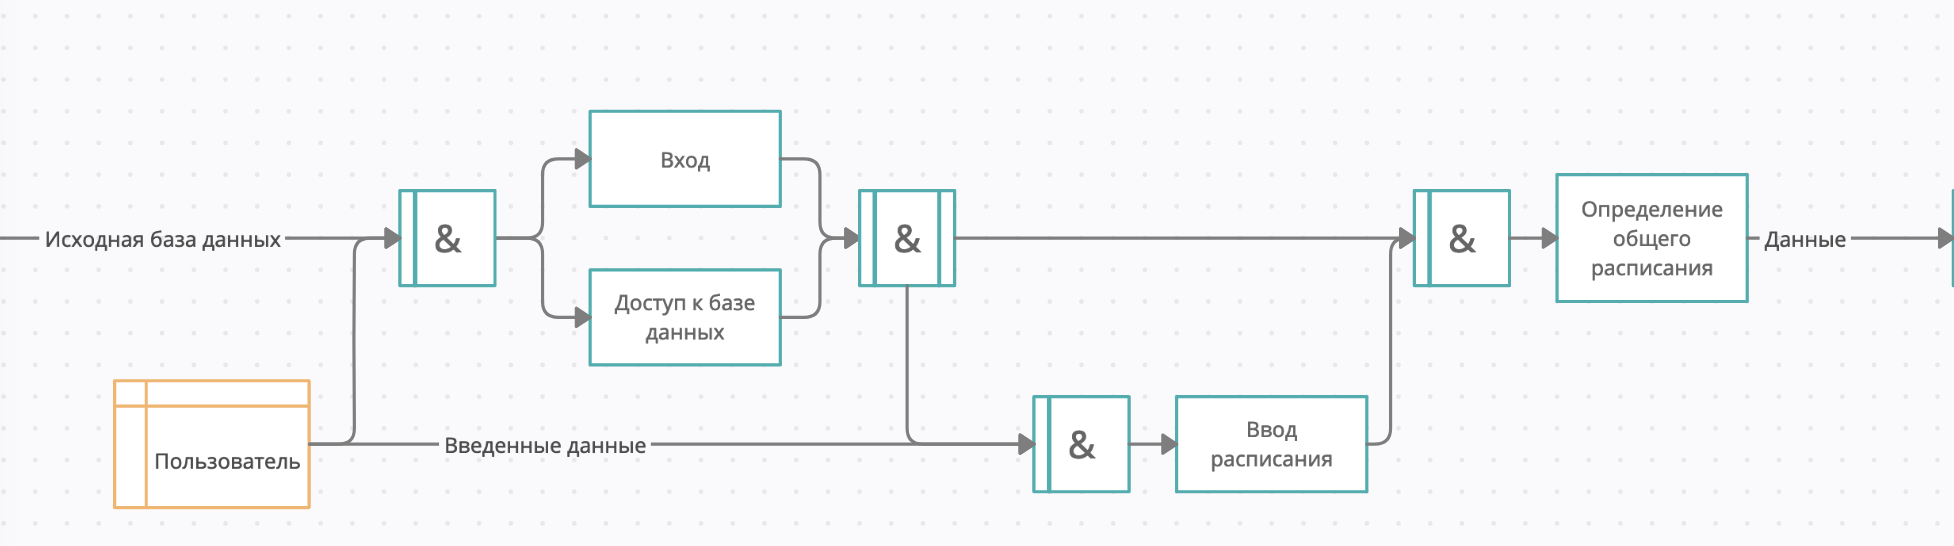
\includegraphics[width=0.7\linewidth]{img/IDEF3-1-0.png}
        \caption{ Декомпозиция контекстной диаграммы по стандарту IDEF3}
        \label{fig:idef32}
    \end{figure}

    \begin{figure}[h]   
        \centering
        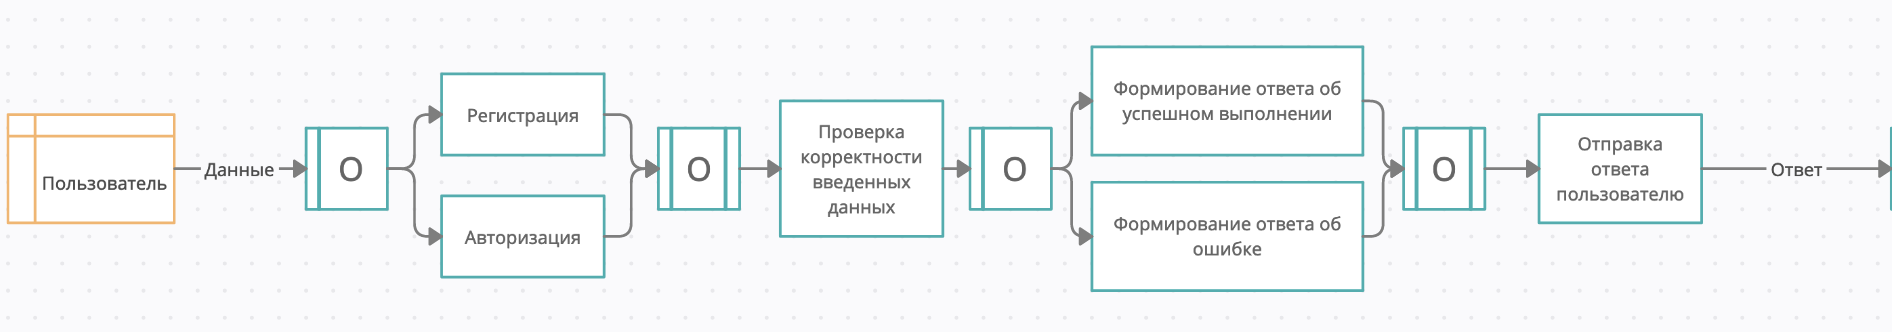
\includegraphics[width=0.9\linewidth]{img/IDEF3-2-0.png}
        \caption{ Декомпозиция блока <<Вход>> по стандарту IDEF3}
        \label{fig:idef33}
    \end{figure}

    \begin{figure}[h]   
        \centering
        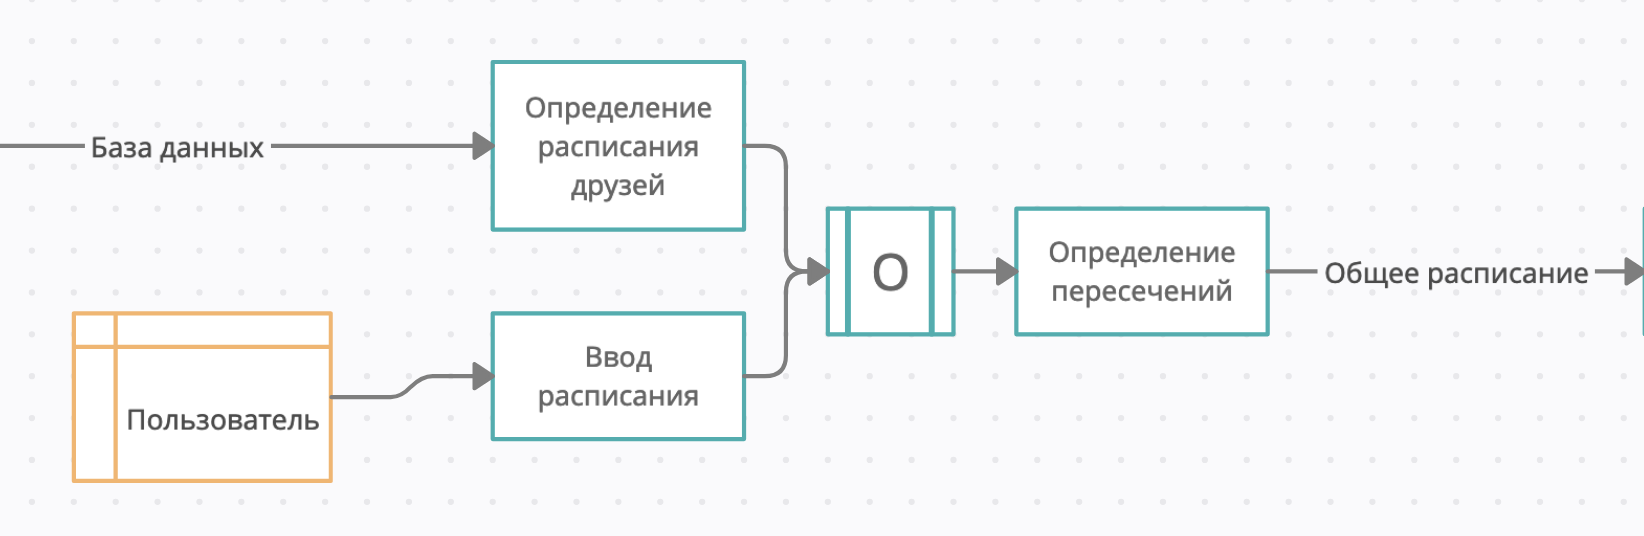
\includegraphics[width=0.9\linewidth]{img/IDEF3-2-1.png}
        \caption{ Декомпозиция блока <<Определение общего расписания>> по стандарту IDEF3}
        \label{fig:idef34}
    \end{figure}
\end{landscape}

\section{Модель процесса в нотации BPMN}
В данном разделе представлена модель процесса в нотации BPMN (рисунок \ref{fig:bpmn})
\begin{figure}[h]   
    \centering
    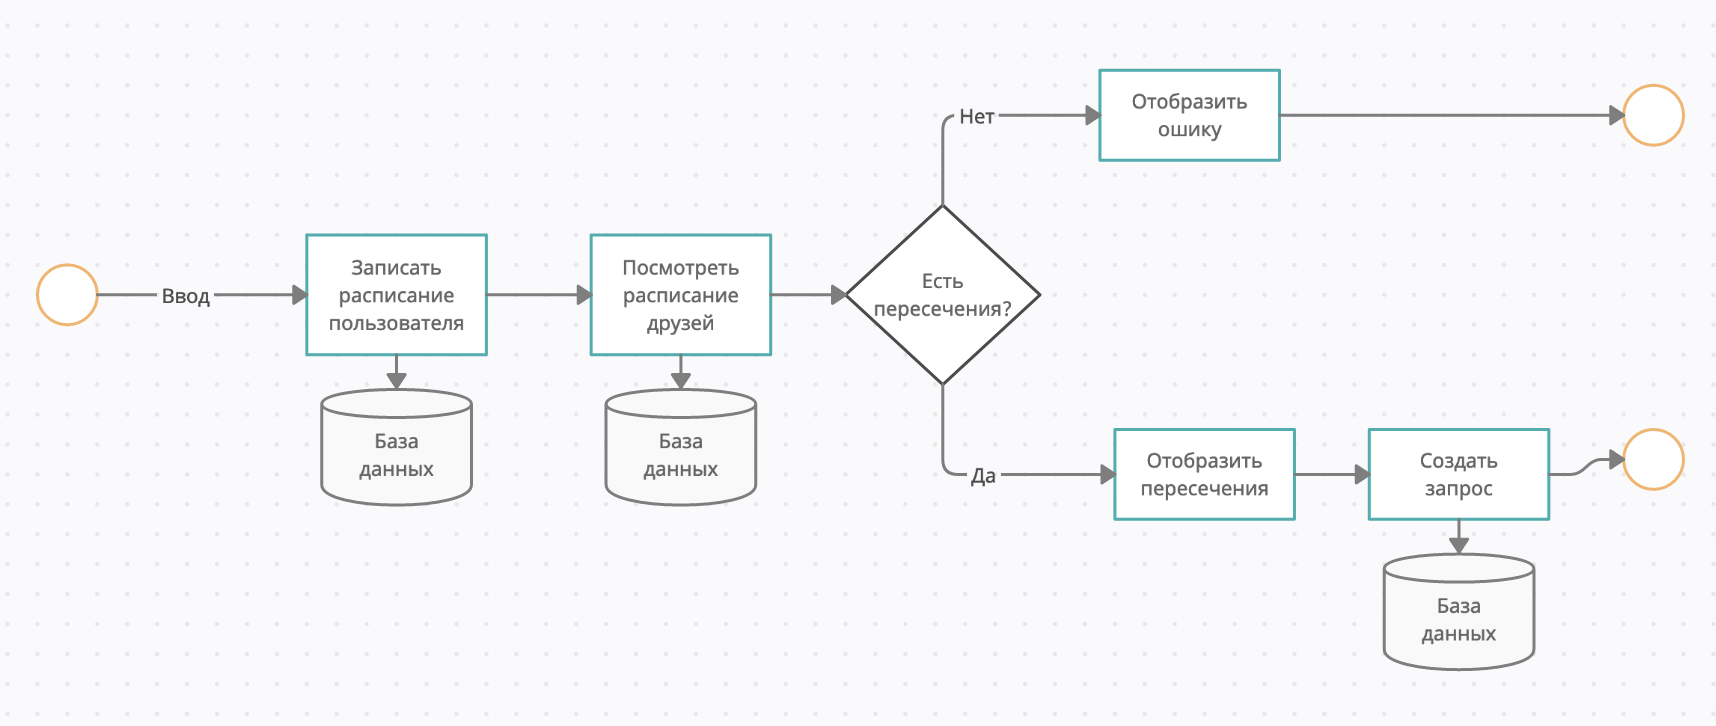
\includegraphics[width=0.9\linewidth]{img/BPMN.png}
    \caption{ Модель по стандарту BPMN}
    \label{fig:bpmn}
\end{figure}




% ////////////////////////////////////////////////////////
%                     ЛАБА 8
% ////////////////////////////////////////////////////////
\chapter{Разработка технического задания на создание инфокоммуникационной системы} 

\section{Общие сведения}
    \subsection{Наименование инфокоммуникационной системы}
        Наименование разрабатываемого программного обеспечения: meet\textunderscore me. 
    \subsection{Сроки начала и окончания работ по созданию инфокоммуникационной системы}
        После заключения договора с Заказчиком, исполнитель обязуется выполнить все работы по созданию инфокоммуникационной системы в течении 90 рабочих дней.

\section{Назначение и цели создания системы}
    \subsection{Назначение системы}
        Информационная система meet\textunderscore me предназначено для планирования встреч с друзьями и родственниками в виде календаря. 
        Система показывает пересечение свободного времени пользователя с одним или несколькими его друзьями.
        C помощью данной системы пользователь может эффективно планировать встречи со своими друзьями, родственниками или знакомыми.

    \subsection{Цели системы}
        Разрабатываемая  система имеет следующие цели:
        \begin{itemize}
            \item Учет пользовательского расписания
            \item Выявление пересечений расписания пользователя с другими пользователями 
            \item Планирование встреч с другими пользователями 
        \end{itemize}

\section{Характеристика объектов автоматизации}
        Объектом автоматизации является выявление пересечений расписания пользорвателя с другими пользователями посредством использование веб приложения.
        
        Веб приложение представляет из себя клиент-серверное приложение в виде веб-сайта для клиентской стороны, программного обеспечения работающего на сервеной части приложения, а так же системы управления базами данных.

\section{Требования к системе}

        \subsection{Требования к отказоустойчивости}
            Разрабатываемая инфокоммуникационная система должна быть отказоусточивой. Система должна выдерживать до 10000 одновременных пользователей. На всех уровнях обработки информации должна быть предусмотрена обработка ошибок. Действия обычного пользователя не должны выводить из строя систему. Необходимо предусмотреть возможные действия недобросовесных пользователей. 

        \subsection{Требования к интерфейсу}
            Разрабатываемый интерфейс должен быть построен согласно стилистическим нормам и должен быть максимально удобен для пользователя. Необходимо разработать интерфейсы следующих размеров (пикс.):
            \begin{itemize}
                \item 375x667
                \item 375x812 
                \item 390x844
                \item 414x896
                \item 810x1080
                \item 1280x720
                \item 1920x1080
                \item 2048x1080
                \item 3840x2160
            \end{itemize}

            Все интерфейсы должны выглядеть в едином стиле и иметь одинаковый функционал. Элементы управления системой должны быть расположены в интуитивно понятных для пользователя местах. Каждый элемент управления должен быть понятно обозначен и должен иметь лишь одну интерпретацию. Для системы следует разработать 2 цветовых гаммы, в светлых и темных тонах. Необходимо реализовать возможность быстро переключаться между цветовыми гаммами. Интерфейс должен выглядеть одинаково для следующих версий программного обеспечения:

            \begin{itemize}
                \item Google Chrome версии 57 или выше;
                \item Edge версии 16 или выше;
                \item Safari версии 11 или выше;
                \item Firefox версии 52 или выше; 
                \item Opera версии 44 или выше;
                \item Остальные браузеры на базе Chromium версии 57 или выше;
            \end{itemize}

            Поддержка семейства браузеров Internet Explorer не требуется. Для неподдерживаемого программного обеспечения необходимо уведомить пользователя о невозможности продолжения работы и предложить ему один из вариантов поддерживаемого программного обеспечения. 

            Интерфейс требуется реализовать в соответствии с представленным макетом интерфейса (Рисунок \ref{fig:prototype}). 
     
        \subsection{Требования к уровню безопасности}
            
            Для информационной системы требуется высокий уровень безопасности и защиты от несанкционированного доступа. Необходимо разработать механизмы двухфакторной аутентификации для пользователей с помощью генерации одноразовых паролей или аппаратных ключей. Необходимо отслеживать подозрительные попытки входа в аккаунт пользователя и своевременно уведомлять его об этом посредством e-mail. Предусмотреть действия недобросовесных пользователей такие как: SQL инъекции, внедрение вредоносного кода путем загрузки файлов, перебор паролей, многократные попытки входа и тд. 

        \subsection{Требования к программному обеспечению}

            В процессе разработки инфокоммуникационной системы необходимо использовать программное обеспечение с открытым исходным кодом и лицензиями MIT, BSD, GLP. В случае невозможности использовать программное обеспечение для той или иной задачи, необходимо согласовать с Заказчиком приобретение лицензии на проприетарное программное обеспечение и его дальнейшее использование. Для управлением базами данных требуется использование нереляционной системы управления базами данных. В качестве системы управления базами данных разрешается использовать проприетарное программное обеспечение MongoDB Enterpise версии 6.0 или выше. Выбранное программное обеспечение должно поддерживать и стабильно функционировать на операционной системе с открытым исходным кодов Ubuntu Server версии 21.10 или выше.  
        \subsection{Требования к техническому обеспечению}

            В процессе разработки интерфейса инфокоомуникационной системы необходимо использовать веб-фреймворк React в совокупности с библиотеками React-router, Redux. Необходимо использовать компонентый подход с использованием библиотеки Styled Components. 

            В процессе разработки серверной части инфокоммуникационной системы необходимо использовать микросервисную архитектуру. Программное обеспечение должно быть масштабируемым. Программное обеспечение должно быть способно обрабатывать до 30000 запросов в секунду. Каждый модуль должен быть покрыт тестами. Так же вся инфокоммуникационная система должна быть пократа интеграционными тестами. В процессе разработки программного обеспечения необходимо избегать дублирования кода. Реализовать серверную часть необходимо с использованием эффективных, современных и поддерживаемых технологий на усмотрение Исполнителя. 

            

        \subsection{Требования к функциям, выполняемым системой}

            Разрабатываемая информационная система должна выполнять функции представленные ниже. 
            \subsubsection{Авторизация пользователя}
                При запуске приложения пользователю необходимо представить возможность войти в уже существующий аккаунт или создать новый. Для создания аккаунта пользователю необходимо ввести следующую информацию:

                \begin{itemize}
                    \item Имя 
                    \item Адрес электронной почты 
                    \item Пароль 
                \end{itemize}

                При создании нового аккаунта или входа в уже существующий, пользователю требуется пройти проверку через сервис Google ReCaptcha. Требуется реализовать обязательное подтверждение адреса электронной почты после регистрации аккаунта. Необходимо реализовать возможность восстановления утраченного пользователем пароля с помощью адреса электронной почты указанного при регистрации. 

            
            \subsubsection{Настройка пользовательского расписания}

                Необходимо реализовать возможность ввода расписания пользователем. Пользователю должны быть доступны следующие действия: 
                \begin{itemize}
                    \item Создание блока времени;
                    \item Удаление блока времени;
                    \item Изменение временного диапазона блока;
                    \item Установка повторения блока с определенной периодичностью;
                \end{itemize}

                Необходимо предусмотреть ввод пользователем некорректных данных и обработать соответствующие ошибки. Требуется реализовать возможность импорта файлов .cal, а так же интеграцию с популярными интернет-сервисами по типу Google Calendar, Proton Calendar и т. д. На основе импортированных данных необходимо подсказывать пользователю, когда у него в расписании может быть свободное время для встреч с другими пользователями информационной системы. 

            \subsubsection{Отправка и принятие заявок в друзья} 
                Для инфокоммуникационной системы необходимо реализовать возможность добавления других пользователей в список друзей. Необходимо реализовать импорт списка друзей из популярных интернет сервисов таких как: Facebook, VK, Google+ и так далее. Реализовать возможность поиска других пользователей по адресу электронной почты указанному при регистрации. Необходимо давать доступ пользователю к расписанию других пользователей только после одобрения заявка другим пользователем. Уведомления о входящих заявках необходимо так же дублировать пользователям с помощью email рассылки. 

            \subsubsection{Создание группы из существующих друзей}
                Для разрабатываемой системы необходимо реализовать возможность создания группы из уже существующих друзей. Для группы необходима возможность коммуницировать между собой в формате коротких сообщений. Так же необходима возможность прикреплять к сообщениями фотографии, геометки, гиперссылки, а так же создавать опросы. Необходимо реализовать возможность участия в опросах только для пользователей соответствующей группы. Заявку на добавление в группу так же необходимо подтвердить соответствующему пользователю. 

            \subsubsection{Отображение общего свободного времени}
                Необходимо реализовать возможность отображения общего свободного времени для инфокоммуникационной системы. Общее свободное время является пересечением свободного времени пользователя с другими пользователями из списка его друзей. Если у пользователя не задано его расписание, необходимо предложить ему настроить свое расписание используя соответствующий функционал. При отображении общего свободного времени для групп пользователей необходимо реализовать отображение количества совпадений с расписаниями других пользователей. Необходимо предоставить возможность пользователю выбирать режим отображения календаря по дням или по неделям или по месяцам. 
                
            \subsubsection{Создание встречи}

                Разрабатываемая инфокоммуникационная система должна иметь функцию создания встреч. Пользователь должен иметь возможность отправить другому пользователю запрос на встречу только при наличии в расписании общего свободного времени. Пользователям должны приходить уведомления о приглашениях в интерфейсе программы, а так же на электронную почту. Пользователь должен иметь возможность принять или отклонить предложение другого пользователя. Для групповых встреч должен быть реализован функционал голосования. 



\section{Состав и содержание работ по созданию системы}

        Разработка инфокоммуникационной системы должна происходить в несколько этапов:
        \begin{enumerate}
            \item Разработка \begin{itemize}
                \item Проработка деталей инфокоммуникационной системы;
                \item Разработка дизайна интерфейса;
                \item Проектирование базы данных;
                \item Разработка серверной стороны приложения; 
                \item Разработка клиентской части приложения;
            \end{itemize}
            \item Тестирование \begin{itemize}
                \item Написание тестов для автоматизированного тестирования;
                \item Ручное тестирование;
            \end{itemize}
            \item Отладка 
            \item Ввод в действие \begin{itemize}
                \item Настройка и ввод в эксплуатацию серверного оборудования;
                \item Настройка программного обеспечения для функционирования инфокоммуникационной системы;
            \end{itemize}
        \end{enumerate}

\section{Порядок контроля и приемки системы} 
    Контроль выполнения производится следующим образом:
    \begin{itemize}
        \item автоматическое модульное тестирование;
        \item автоматическое интеграционное тестирование;
        \item тестирование безопасности программного обеспечения установленного на серверном оборудовании;
        \item тестирование безопасности веб-приложения;
        \item тестирование веб-приложения на нагрузки;
        \item ручное тестирование;
        \end{itemize}

    Ответственность за организацию приемки несет Заказчик. Исполнителю необходимо предоставить заказчику технические средства, проектную документацию и технический персонал.

    Конечным этапом является составление между Заказчиком и Исполнителем акта приемки. 

\section{Требования к составу и содержанию работ по подготовке объекта автоматизации к вводу системы в действие}
    Для ввода в действие инфокоммуникационной системы Исполнитель обязан провести следующие действия:
    \begin{itemize}
        \item Покупка серверного оборудования;
        \item Заключение договора с центром обработки данных на размещение серверного оборудования;
        \item Настройка серверного оборудования;
        \item Настройка программного беспечения на серверном оборудовании;
        \item Приобретение доменного имени и настройка соответствующих записей;
    \end{itemize}

\section{Требование к документированию}
    Для информационной системы должна быть разработана документация согласно ГОСТ 34. Документация должна включать в себя: 
    \begin{itemize}
        \item Техническая документация на код, алгоритмы, интерфейсы и API;
        \item Проектная документация;
        \item Пользовательская документация;
    \end{itemize}
    Документация должна быть выполнена на русском языке. Документация должна быть передана Заказчику в электронном виде в формате pdf (Portable Document Format).

\section{Источники разработки}
    Данное техническое задание разработано на основе документа ГОСТ 34.602-89 <<Информационная технология. Комплекс стандартов на автоматизированные системы. Техническое задание на создание автоматизированной системы.>>



\conclusions
В процессе работы над курсовой работой была достигнута поставленная цель, а так же:
\begin{itemize}
    \item описана идея системы 
    \item проведен анализ рынка 
    \item разработаны диаграммы согласно стандартам UML, IDEF0, IDEF3, DFD, BPMN для описания принципов функционирования системы.
    \item создано техническое задание на разработку инфокоммуникационной системы;
\end{itemize}

При написании курсовой работы был получен опыт в оформлении официальных работ, написании технического задания, проектирование моделей систем согласно различным стандартам. Курсовая работа, полученный опыт и знания помогут в дальнейшем развитии инфокоммуникационной системы MEET ME.

\newpage
\begin{thebibliography}{99}
    \item \label{a:NeetToMeet} NeedToMeet: официальный сайт. URL: \url{https://www.needtomeet.com} (Дата обращения 19.10.2022)
    \item \label{b:Rally} Rally: официальный сайт. URL: \url{https://rallly.co/} (Дата обращения 19.10.2022)
    \item \label{c:WhenAvalible} WhenAvalible: официальный сайт. URL: \url{https://whenavailable.com/} (Дата обращения 19.10.2022)
    \item \label{bib1} В. И. Горбаченко. <<СОЗДАНИЕ ФУНКЦИОНАЛЬНОЙ МОДЕЛИ ИНФОРМАЦИОННОЙ СИСТЕМЫ С ПОМОЩЬЮ CASE-средства CA ERwin Process Modeler 7.3>> - Пенза 2010 - 25-55с.
	\item \label{bib2} 	UML Use Case Diagram Tutorial | Lucidchart URL: \url{https://www.lucidchart.com/pages/uml-use-case-diagram} (Дата обращения \today)
    \item \label{bib3} 	UML Activity Diagram Tutorial | Lucidchart URL: \url{https://www.lucidchart.com/pages/uml-activity-diagram} (Дата обращения \today)
    \item \label{bib4} ГОСТ 34.602-89. Информационная технология. Комплекс стандартов на автоматизированные системы. Техническое задание на создание автоматизированной системы.

\end{thebibliography}

\end{document}
